\chapter{Introducción Específica} % Main chapter title

\label{Chapter2}

%----------------------------------------------------------------------------------------
%	SECTION 1
%----------------------------------------------------------------------------------------

En este capítulo se hará énfasis en las características de la experiencia en la que se utilizará el equipo y sus necesidades. Esto da origen a cada uno de los requerimientos de diseño.

Este proyecto se destaca principalmente por ser un sistema de adquisición diseñado especialmente para realizar experiencias en animales grandes sin alterar su comportamiento durante lapsos prolongados, para evitar incidir sobre los valores de tensión arterial medidos. Para ello, el desarrollo se enfocó en lograr un equipo de pequeño tamaño y bajo peso, y a la vez se trabajó en la necesidad de contar con una interfaz de usuario inalámbrica que permita configurar el equipo y chequear esporádicamente su funcionamiento evitando que el operador se acerque al animal. 

El equipo diseñado digitaliza las señales analógicas y las guarda en una memoria flash de almacenamiento masivo (SD) durante períodos de tiempo prolongados, de aproximadamente 24hs. Puede configurarse y controlarse desde una terminal remota a través de una interfaz comunicada por BLE.

\section{Detalle de las necesidades}

Las experiencias de medición consisten básicamente en colocar el equipo en una especie de pequeña mochila que se ajusta sobre el animal instrumentado con sensores de presión intra-arteriales. Una vez instalado, el equipo digitaliza y adquiere las señales provenientes de los dos sensores durante un período de 24hs. Esto da un margen de tiempo para que el animal se tranquilice luego de la instalación del dispositivo, normalice su comportamiento, y pase por diferentes fases a lo largo del día: vigilia, sueño, alimentación, interacción con veterinarios, etc. 

La presión arterial es un parámetro que es fuertemente dependiente del bienestar del animal, por lo que es importante que la batería tenga autonomía suficiente para toda la experiencia y que no sea necesario un recambio o recarga. Es necesario que sea portátil para que el animal no esté conectado a ningún equipo a través de cables. Como se trata de una experiencia larga, también es importante que el equipo no sea pesado, voluminoso, ruidoso, ni se caliente. 

Los sensores utilizados son del tipo strain-gauge. Pueden visualizarse en la imagen \ref{fig:konigsberg}. Se trata de una resistencia que varía su valor de acuerdo a la presión aplicada. El sensor además cuenta con propiedades aptas para ser implantado en un animal. Este sensor tiene un conector propio de la marca Königsberg al que se le conecta un compensador por temperatura calibrado específicamente para cada sensor, y de allí se utiliza un conector estándar roscado Amphenol de 4 pines dorados para ingresar al equipo. Esta última conexión es muy importante para evitar que se agregue ruido a la señal medida.

\begin{figure}[!htbp]
	\centering
	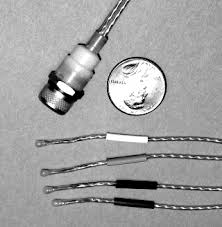
\includegraphics[width=\textwidth]{./Figures/konigsberg.jpeg}
	\caption{Imagen de conector, cable y sensor Königsberg}
	\label{fig:konigsberg}
\end{figure}

La señal de presión arterial tiene un patrón normal con diferentes puntos característicos. Puede observarse en la figura \ref{fig:senpresion} un gráfico típico de una señal de presión arterial de un mamífero. La forma de la curva corresponde a una onda estacionaria conformada por una señal incidente pulsátil y una onda reflejada, y puede analizarse como un sistema de parámetros distribuídos. 

Desde el punto de vista del análisis frecuencial, la señal de presión tiene una frecuencia fundamental apenas superior a 1 Hz, sin embargo, contiene componentes de hasta los 100 Hz, con los que es necesario contar para obtener una buena resolución en el momento de realizar el análisis de la forma de onda. Una frecuencia de muestreo típica utilizada para adquirir este tipo de señales es \textbf{500 Hz} o \textbf{1 kHz}. Una excursión normal de una señal de presión de un ser humano puede tener un máximo de 140mmHg, por lo que es útil contar con un rango dinámico mayor a este, por ejemplo 200 mmHg. Una adquisición con una resolución del 0.5\%, es decir, de 1 mmHg sería adecuada.

\begin{figure}[!htbp]
	\centering
	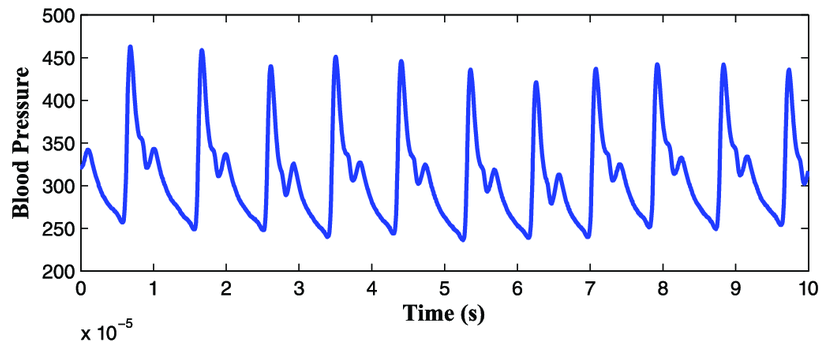
\includegraphics[width=\textwidth]{./Figures/senpresion.png}
	\caption{Señal típica de presión arterial de un mamífero.}
	\label{fig:senpresion}
\end{figure}

Es muy común que antes de comenzar la experiencia, o durante la experiencia, el animal se mueva o intente tocar los cables que van desde los sensores hasta la mochila donde se encuentra alojado el equipo. Estos movimientos pueden ocasionar cambios en el estado de las conexiones de los sensores, o eventualmente, en el estado del equipo. Es útil, desde el punto de vista del operador del equipo, poder tener algún tipo de información sobre la señal que se está midiendo, de manera de saber si es necesario realizar algún ajuste en las conexiones. Sin embargo, esta observación se debe poder realizar sin molestar al animal, es decir en forma inalámbrica. También es importante compensar una eventual pérdida de ganancia analógica por movimiento de los sensores para no ver disminuída la resolución de la adquisición. 

Finalmente, una vez comenzada la medición, al tratarse de una experiencia tan costosa en cuanto a recursos y tiempo, es importante poder controlar esporádicamente que la adquisición se esté realizando de forma correcta, sin afectar el comportamiento del animal. Por lo tanto es muy útil desde el punto de vista operativo de recursos poder visualizar la señal que se está adquiriendo en forma remota sin influir en el animal, es decir, de forma remota.


\section{Requerimientos}

En base a todo lo comentado en la sección anterior, se desprenden los siguientes requerimientos asociados de acuerdo a criterios de energía, tamaño y peso, conectividad y adquisición, con los que fue desarrollado el equipo:


\begin{enumerate}
	\item \textbf{Necesidades asociadas a la alimentación:} 
	\begin{enumerate}
		\item El equipo debe tener una autonomía mayor a 24 horas en el modo de adquisición y almacenamiento, a una dada frecuencia de muestreo.
		\item El equipo debe ser portátil e inalámbrico, por lo tanto, alimentado a batería
	\end{enumerate}
	
	\item \textbf{Requerimientos asociados al tamaño físico del equipo:}
	\begin{enumerate}
		\item El peso del equipo debe tener un peso aproximado de 500 gr
		\item El tamaño debe ser aproximadamente de 10cm x 10cm
		\item El equipo no debe calentarse demasiado
	\end{enumerate}
	
	\item \textbf{Requerimientos asociados a la conectividad e interfaz de usuario:}
	
	\begin{enumerate}
		\item Se deben poder visualizar las señales medidas en tiempo real previo a iniciar la experiencia.
		\item Se debe realizar la configuración de la adquisición (ganancia, canales habilitados, frecuencia de muestreo, etc.) desde una terminal Bluetooth.
		\item Se debe poder acceder a la memoria SD a través de la conexión USB.
	\end{enumerate}


	\item \textbf{Requerimientos asociados a la adquisición y almacenamiento:}
	
	\begin{enumerate}
		\item El equipo debe tener una resolución de 1 mmHg en alguna de las escalas de ganancia.
		\item Debe poder manejar almacenamiento suficiente para la máxima resolución elegida y frecuencia de muestreo.
		\item Se debe poder configurar el tamaño de muestra.
	\end{enumerate}

\end{enumerate}


\section{Planificación}

En las siguiente figura \ref{fig:gantt}  puede observarse la planificación original del trabajo en un diagrama de Gantt. 

\begin{sidewaysfigure}
	\centering	
	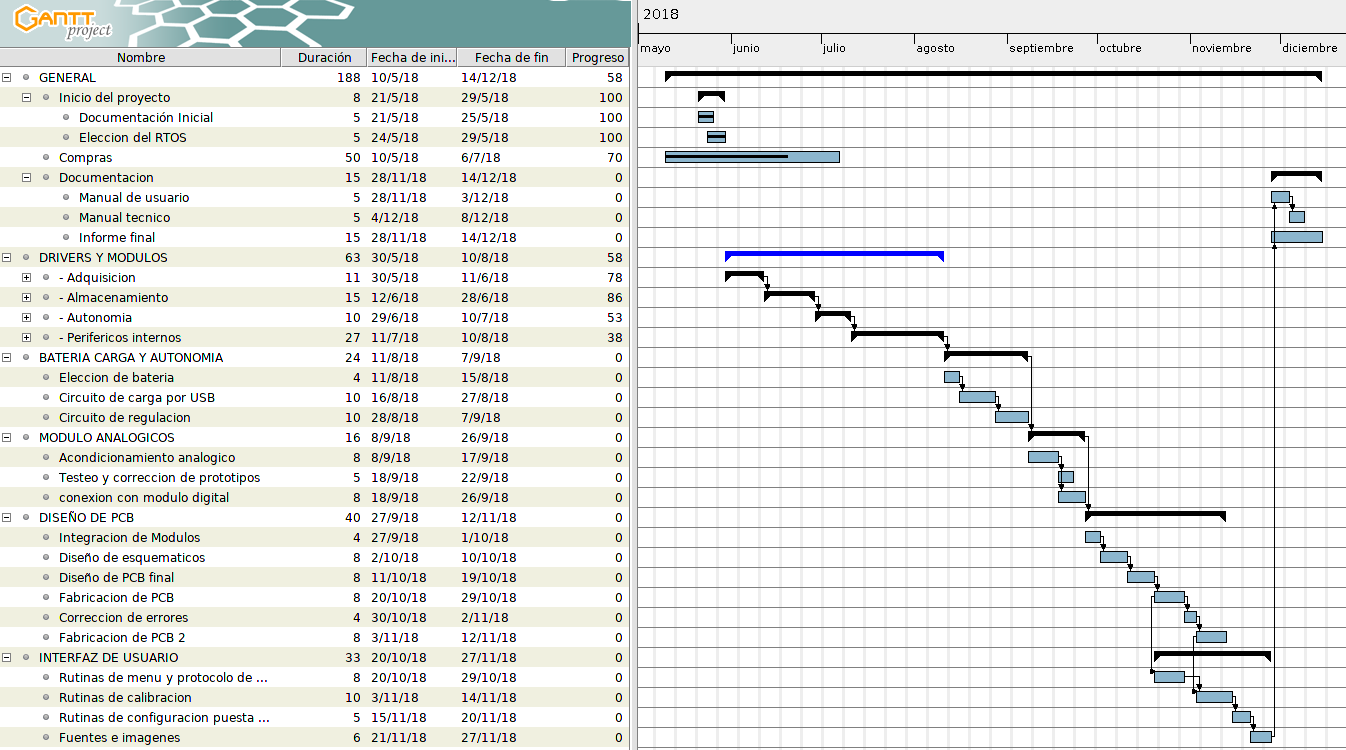
\includegraphics[width=\textwidth]{./Figures/gantt.png}
	\caption{Diagrama de gantt - Primer parte}
	\label{fig:gantt}
\end{sidewaysfigure}

En este diagrama puede verse la organización del trabajo separado en los siguientes módulos:

\begin{enumerate}

\item \textbf{General:} Documentación inicial del proyecto, selección de rtos y microcontrolador, documentación de memoria técnica, manuales de usuario y técnico, presentaciones, compras de componentes, pedido de servicios, etc.

\item \textbf{Drivers y módulos:} driver del ADC, tests de adquisición, driver de almacenamiento, manejo del DMA, interfaz de prueba para configuración, programación de drivers de periféricos, etc.

\item \textbf{Batería, carga y autonomía:} medición de consumo, elección de batería, circuito de carga USB, circuito de regulación.

\item \textbf{Módulos analógicos:} acondicionamiento analógico de la señal, interconexión con módulo digital.

\item \textbf{Diseño de PCB:} integración de módulos, esquemáticos, diseño de PCB, fabricación, soldadura, etc.

\item \textbf{Interfaz de Usuario:} Rutinas de menú, protocolo de comunicación, configuración, fuentes, imágenes, testing unitarios, testing de sistema, etc.

\end{enumerate}